%% LaTeX2e class for student theses
%% sections/2_chapter/req_eng_and_pr_design.tex
%%
%% Karlsruhe University of Applied Sciences
%% Faculty of  Computer Science and Business Information Systems
%%
%% --------------------------------------------------------
%% | Derived from sdqthesis by Erik Burger burger@kit.edu |
%% --------------------------------------------------------

\chapter{Requirements Engineering and Process Design}
\label{ch:Requirements Engineering and Process Design}

Based on the existing concepts and design proposals elaborated in the previous chapter, this work has the target to design and implement a reservation process considering a problem statement described in detail as part of the following section. 
After an analysis of the identified actors and use cases of the outlined scenario, requirements for the process design will be derived and formalized in diagrams with the Business Process Modelling Notation \cite{noauthor_bpmn_nodate} and Unified Modelling Language 2.0 \cite{noauthor_welcome_nodate}.
Resulting in a reservation process design describing the interactions with its users and the behavior in different situations will stay at the end of this chapter. 

\section{Scenario}
\label{ch:Requirements Engineering and Process Design:sec:Scenario}

For the conceptional design of the process a scenario will be used, to simulate different actors and their needs with regard to the criteria of usability and accessibility. Afterwards these actors will be used as personas to formulate use cases and the interactions with the system. 
Beginning with the selection of the location, the subsequent setting takes place. Appropriate to its functionality as partner of the underlying project, which is artifact of this work, the \acrfull{hka} with focus on three of the site areas within the city of Karlsruhe is selected.
The designation and the location within the city are irrelevant for this scenario and will not be further described.
Each site represents a separate campus with the corresponding students, their lecturers and staff of the \acrshort{hka}, which use different transport facilities to bridge the distance between the campuses themselves or their homes. 
Beside the people arriving via public transport, the author assumes that in case of subventions of electric vehicles in the federal republic of Germany, a growing amount of people have acquired electric vehicles for their daily transportation. 
The parking lots at the different campus sites offer a limited amount of \acrfull{cs}s to provide charging capabilities to a subset of \acrfull{evu}s arriving there. 
Regarding the management of the existing charging infrastructure, the \acrshort{hka} uses an open source solution, which consists of a user interface accessible through a browser and used by administrative departments of the different campuses, a mobile client for the end users and a backend system procuring the communication with the facilities. 
By now, the administrator or the end user does not have an opportunity to reserve a charging station connector on behalf of a specific user or for themselves.
Just the enabling and disabling of specific charging connectors or the whole charging station is implemented.
As an implication of this restriction, a "first-come-first-serve" mentality among the \acrshort{evu}s will be induced and a equitable usage of the existing charging possibilities is not given anymore.
To prohibit such a invidious situation the mentioned solution should furnish a reservation functionality allowing a fine grained distribution between public accessible \acrshort{cs} connectors and a subset, which is prohibited for public use and for \acrshort{evu}s with existing reservations only.

\subsection{Actors}
\label{ch:Requirements Engineering and Process Design:sec:Scenario:ssec:Actors}

Next, the scenario needs a set of actors, which could be used as personas for describing different use cases, the system has to provide in case of an interaction with the given actor. 
In case of a university, as described above, the author selected a subset of possible groups of people, existing in such a context. 
Therefore, four groups were selected, representing a required minimum for constructing viable cases and edge cases. Each group has a representative in form of a persona, pictured by a fictional person in combination with a role inside the system itself.
For a better understanding of the role collection provided by the system, the following table \ref{tab:system_role_collection} introduces the relevant roles, shortages and a brief description.

\begingroup
\setlength{\tabcolsep}{10pt} % Default value: 6pt
\renewcommand{\arraystretch}{1.5} % Default value: 1
\begin{table}[h!]
    \centering
    \begin{tabular}{c|c|c|m{6cm}}
        Role & System & Shortage & Description \\
        \hline
        Basic & \verb|BASIC| & \verb|B| & Standard user without administrative privileges \\
        Admin & \verb|ADMIN| & \verb|A| & User with administrative privileges inside a tenant organisation \\
        Super Admin & \verb|SUPER_ADMIN| & \verb|S| & User with extended administrative privileges for creation of tenant organizations and initialization of templates for cars and charging stations \\
        Demo & \verb|DEMO| & \verb|D| & Demo user for test purposes \\
    \end{tabular}
    \caption{Role collection provided by the system}
    \label{tab:system_role_collection}
\end{table}
\endgroup

The identified groups of the scenario will be part of the next listing. Therefore, the group will be described and in the next step assigned to a specific role in the context of the case.

\begin{description}
    \item[Student] Personas representing students studying at the \acrshort{hka}. Mainly they spent time at the main campus, where all lectures and the attendant exercises take place. To travel between their home and the university, beside using the train, they drive with electric vehicles or plug-in hybrids to minimise their carbon footprint. Due to the fact, that the amount of students with EVs outnumber the capacity of charging stations at the different sites of the \acrshort{hka}, this group does not have the possibility to reserve a charging station for recharging their vehicles. Students have to arrive early to catch one of the charging points, which are free/public available.
    \item[Staff] Set of personas belonging to the staff of \acrshort{hka}. They have different roles inside the university, which could be lecturer, service worker, cleaner or librarian for example. Unlike students, the staff has the option to request a reservation. This reservation request will be processed by the secretary of the institution or directly via the janitor. By permitting the request the staff members get a reservation for a charging point/connector at the specified site of \acrshort{hka}. In case of days of or working from home, the reservations could be canceled. Otherwise the janitor or the secretaries could do this via the CSMS admin dashboard. As a rule of thumb this kind of reservations are recurring.
    \item[Janitor] This group represents a special subset of \acrshort{hka} staff. Beside managing and maintaining parts of the physical infrastructure, they are responsible for service offerings regarding the charging stations installed on the three different campus locations. To observe the connected infrastructure, they have access to the administration dashboard provided by the open source solution and are responsible for handling incoming reservation requests. 
    \item[Secretary] In contrast to the group of janitors, the secretary is the administrative counterpart for managing the data and internal processes inside the \acrshort{hka}. Beside paperwork regarding approvals for new students, updating the annual records and processing requests from students, they are organizing events and supervise external visitors. Therefore, staff members inside the secretary needs occasionally access to the charging station management platform to guarantee charging possibilities to guests arriving at the different campus locations.
\end{description}

\begin{table}[h!]
    \centering
    \begin{tabular}{c|c}
        Group & Role \\
        \hline
        Student & \verb|BASIC| \\
        Staff & \verb|BASIC| \\
        Janitor & \verb|ADMIN| \\
        Secretary & \verb|ADMIN|
    \end{tabular}
    \caption{Role mapping of the system roles to the different groups identified in the scenario described in \ref{ch:Requirements Engineering and Process Design:sec:Scenario}}
    \label{tab:role_mapping_scenario}
\end{table}


\subsection{Personas}
\label{ch:Requirements Engineering and Process Design:sec:Scenario:ssec:Personas}

For a better understanding of the different roles and their requirements they concern by using the system, a set of personas is described below. They will be used as identifier and a representative for the user group they are assigned to. A detailed description of the four different personas and their circumstances follows afterwards.

\subsubsection{Lisa Knaus}
\label{ch:Requirements Engineering and Process Design:sec:Scenario:ssec:Personas:sssec:Lisa Knaus}

Lisa Knaus is a student of the \acrshort{hka}. She studies Computer Science in third semester and lives in her hometown Untergrombach. Since she was 18 years old, she used a car as main transport medium. For travelling between her location to study and her hometown she uses the family car, which is an \acrfull{fev} without an \acrfull{ice}. The battery health of her car allows her to reach the main campus and return home after lectures, without a need to recharge. But occasionally she forgot to charge her car at home and need to recharge her vehicle at the \acrshort{hka}. For using the charging service at the parking lots on-site, she submitted a request for account creation at the secretary of her university. Since then, she uses the offered service from time to time, if she arrives early enough to catch a free charging station.

\subsubsection{Holger Starke}
\label{ch:Requirements Engineering and Process Design:sec:Scenario:ssec:Personas:sssec:Holger Starke}

Holger Starke is part of the maintenance team taking care of the server landscape the \acrshort{hka} hosting its internal applications and fostering their user databases. By virtue of the subvention of electric vehicles by the state and his employer he bought a \acrshort{fev} last year. Despite the fact of his short travelling distance between his apartment in Karlsruhe and his workplace, he does not have the possibility to recharge the \acrshort{ev} at home. So he has to use the available charging stations at the different campus locations the \acrshort{hka} offers. However, sometimes if he has to switch between the different campuses very often, the available \acrshort{cs} are already taken.

\subsubsection{Dieter Krause}
\label{ch:Requirements Engineering and Process Design:sec:Scenario:ssec:Personas:sssec:Tom Krause}

Dieter Krause works as a janitor at \acrshort{hka} for five years now. Before taking over the responsibility for the charging infrastructure management and maintenance he acted as carrier for book orders between the various university libaries in Karlsruhe. For transportation purposes he used a van owned by his employer to gather the book orders at one library and drive them to the others. Because of short traveling distances inside Karlsruhe the \acrshort{hka} provided him \acrshort{fev} for reducing carbon dioxide emissions. To fulfill his new purpose as service worker for the charging stations he could further utilize the old van. In contrast to the other \acrshort{evu}s Tom has the option to charge his van on a exclusive \acrshort{cs}, which is dislocated from the other charging infrastructure. Even at days with high emergence of student vehicles on the public parking lots, he could recharge the batteries of the van. 

\subsubsection{Nadine Funke}
\label{ch:Requirements Engineering and Process Design:sec:Scenario:ssec:Personas:sssec:Nadine Funke}

Nadine Funke is a secretary at the administration office of \acrshort{hka} for three years. Formerly she worked at the public administration office in Karlsruhe and already have experience with the complex of problems regarding the charging of \acrshort{ev}s at public charging infrastructure. Beside the maintenance staff, she got access to the charging station management dashboard for blocking \acrshort{cs}s in consideration of arriving guests. Till now, she has to select the specific charging station and the according connector for blocking and needs to enable it again, if the guest has arrived. 

\subsection{Use Cases}
\label{ch:Requirements Engineering and Process Design:sec:Scenario:ssec:Use Cases}

Analysing the scenario described in \ref{ch:Requirements Engineering and Process Design:sec:Scenario}, the following use cases were identified. In terms of clarity and better understanding of the assignment of use case with persona group, the following use case diagrams are describing the use cases in terms of normal users with the role \verb|BASIC| in separation to the use cases administrative users with the role \verb|ADMIN| care about. Afterwards a detailed description of the single cases will follow.

\begin{figure}[h!]
    \centering
    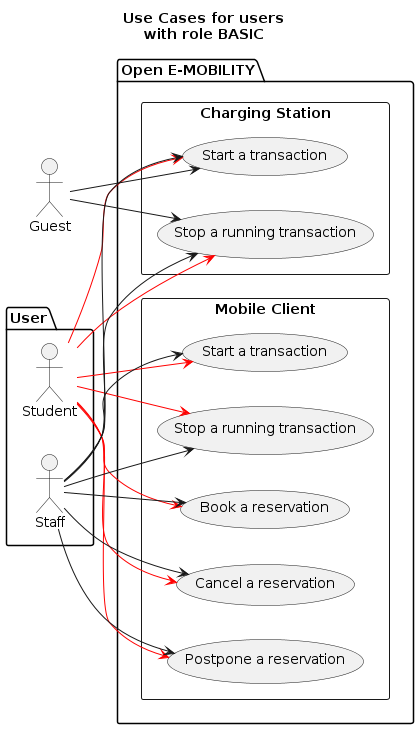
\includegraphics[scale=0.4]{thesis/sections/images/main/2_chapter/uc_basic_users.png}
    \caption{Use Cases for users of Open E-MOBILITY system with role BASIC or as guest user}
    \label{fig:uc_basic_users}
\end{figure}



\begin{figure}[h!]
    \centering
    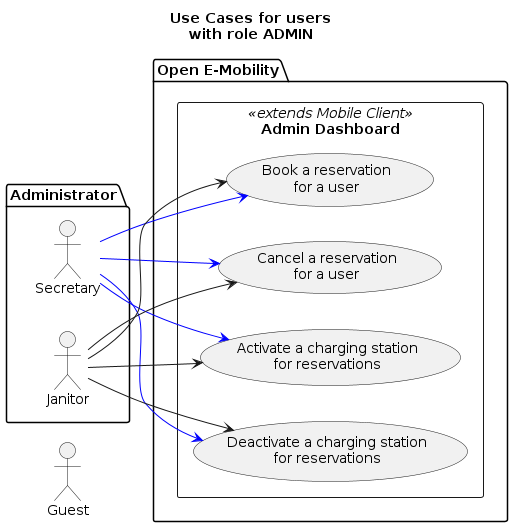
\includegraphics[scale=0.4]{thesis/sections/images/main/2_chapter/uc_admin_users.png}
    \caption{Use Cases for users of Open E-MOBILITY system with role ADMIN or as guest user}
    \label{fig:uc_admin_users}
\end{figure}

\begingroup
\setlength{\tabcolsep}{10pt} % Default value: 6pt
\renewcommand{\arraystretch}{1.5} % Default value: 1
\begin{table}[h!]
    \centering
    \begin{tabular}{m{3.5cm}|c|m{3cm}|m{4cm}}
        Use Case & Shortage & Corresponding Persona & Description \\
        \hline
        Book a reservation & UC1 & Student, Staff, Janitor, Secretary & TODO: \\
        Cancel a reservation & UC2 & Student, Staff, Janitor, Secretary & TODO: \\
        Edit a reservation & UC3 & Student, Staff, Janitor, Secretary & TODO: \\
        Start a transaction & UC4 & Student, Staff, Janitor, Secretary & TODO: \\
        Stop a running transaction & UC5 & Student, Staff, Janitor, Secretary & TODO: \\
        Book a reservation on behalf of another user  & UC6 & Student, Staff, Janitor, Secretary & TODO: \\ 
        Cancel a reservation on behalf of another user & UC7 & Janitor, Secretary & TODO: \\
        Enable charging station for reservation & UC8 & Janitor, Secretary & TODO: \\
        Disable charging station for reservation & UC9 & Janitor, Secretary & TODO: \\
    \end{tabular}
    \caption{Use Case overview with assignment to the corresponding personas and a brief description}
    \label{tab:use_case_overview}
\end{table}
\endgroup

\subsection{System Interactions}
\label{ch:Requirements Engineering and Process Design:sec:Scenario:ssec:System Interactions}

\subsection{Process Design}
\label{ch:Requirements Engineering and Process Design:sec:Scenario:ssec:Process Design}

